%%%%%%%%%%%%%%%%%%%%%%%%%%%%%%%%%%%%%%%%%
% Professional Newsletter Template
% LaTeX Template
% Version 1.0 (09/03/14)
%
% Created by:
% Bob Kerstetter (https://www.tug.org/texshowcase/) and extensively modified by:
% Vel (vel@latextemplates.com)
% 
% This template has been downloaded from:
% http://www.LaTeXTemplates.com
%
% License:
% CC BY-NC-SA 3.0 (http://creativecommons.org/licenses/by-nc-sa/3.0/)
%
%%%%%%%%%%%%%%%%%%%%%%%%%%%%%%%%%%%%%%%%%

\documentclass[9pt]{extarticle} % The default font size is 10pt; 11pt and 12pt are alternatives

%%%%%%%%%%%%%%%%%%%%%%%%%%%%%%%%%%%%%%%%%
% Professional Newsletter Template
% Structural Definitions File
% Version 1.0 (09/03/14)
%
% Created by:
% Vel (vel@latextemplates.com)
% 
% This file has been downloaded from:
% http://www.LaTeXTemplates.com
%
% License:
% CC BY-NC-SA 3.0 (http://creativecommons.org/licenses/by-nc-sa/3.0/)
%
%%%%%%%%%%%%%%%%%%%%%%%%%%%%%%%%%%%%%%%%%

%----------------------------------------------------------------------------------------
%	REQUIRED PACKAGES
%----------------------------------------------------------------------------------------

\usepackage{listings}
\usepackage{graphicx} % Required for including images
\usepackage{microtype} % Improved typography
\usepackage{multicol} % Used for the two-column layout of the document
\usepackage{booktabs} % Required for nice horizontal rules in tables
\usepackage{wrapfig} % Required for in-line images
\usepackage{float} % Required for forcing figures not to float with the [H] parameter
\usepackage[utf8]{inputenc}
\usepackage{fancyhdr}

%------------------------------------------------
% Fonts

\usepackage{charter} % Use the Charter font as the main document font
\usepackage{courier} % Use the Courier font for \texttt (monospaced) only
\usepackage[T1]{fontenc} % Use T1 font encoding

%------------------------------------------------
% List Separation

\usepackage{enumitem} % Required to customize the list environments
\setlist{noitemsep,nolistsep} % Remove spacing before, after and within lists for a compact look

%------------------------------------------------
% Figure and Table Caption Styles

\usepackage{caption} % Required for changing caption styles
\captionsetup[table]{labelfont={bf,sf},labelsep=period,justification=justified} % Specify the table caption style
\captionsetup[figure]{labelfont={sf,bf},labelsep=period,justification=justified, font=small} % Specify the figure caption style
\setlength{\abovecaptionskip}{10pt} % Whitespace above captions

%------------------------------------------------
% Spacing Between Paragraphs

\makeatletter
\usepackage{parskip}
\setlength{\parskip}{6pt}
\newcommand{\@minipagerestore}{\setlength{\parskip}{6pt}}
\makeatother

%----------------------------------------------------------------------------------------
%	PAGE MARGINS AND SPACINGS
%----------------------------------------------------------------------------------------

\textwidth = 7 in % Text width
\textheight = 10 in % Text height
\oddsidemargin = -18pt % Left side margin on odd pages
\evensidemargin = -18pt % Left side margin on even pages
\topmargin = -36pt % Top margin
\headheight = 0pt % Remove the header by setting its space to 0
\headsep = 0pt % Remove the space between the header and top of the page
\parskip = 2pt % Space between paragraph
\parindent = 0.0in % Paragraph indentation
\pagestyle{empty} % Disable page numbering

%----------------------------------------------------------------------------------------
%	COLORS
%----------------------------------------------------------------------------------------

\usepackage[dvipsnames,svgnames]{xcolor} % Required to specify custom colors

\definecolor{altncolor}{rgb}{.8,0,0} % Dark red
%\definecolor{altncolor}{rgb}{.2,.4,.8} % Dark blue
%\definecolor{altncolor}{rgb}{.84,.16,.16} % Red

\usepackage[colorlinks=true, linkcolor=altncolor, anchorcolor=altncolor, citecolor=altncolor, filecolor=altncolor, menucolor=altncolor, urlcolor=altncolor]{hyperref} % Use the color defined above for all links

%----------------------------------------------------------------------------------------
%	BOX STYLES
%----------------------------------------------------------------------------------------

\usepackage[framemethod=TikZ]{mdframed}% Required for creating boxes
\mdfdefinestyle{sidebar}{
    linecolor=black, % Outer line color
    outerlinewidth=0.5pt, % Outer line width
    roundcorner=0pt, % Amount of corner rounding
    innertopmargin=10pt, % Top margin
    innerbottommargin=10pt, % Bottom margin
    innerrightmargin=10pt, % Right margin
    innerleftmargin=10pt, % Left margin
    backgroundcolor=white, % Box background color
    frametitlebackgroundcolor=white, % Title background color
    frametitlerule=false, % Title rule - true or false
    frametitlerulecolor=white, % Title rule color
    frametitlerulewidth=0.5pt, % Title rule width
    frametitlefont=\Large, % Title heading font specification
    font=\small
}

\mdfdefinestyle{intextbox}{
    linecolor=black, % Outer line color
    outerlinewidth=0.5pt, % Outer line width
    roundcorner=10pt, % Amount of corner rounding
    innertopmargin=7pt, % Top margin
    innerbottommargin=7pt, % Bottom margin
    innerrightmargin=7pt, % Right margin
    innerleftmargin=7pt, % Left margin
    backgroundcolor=white, % Box background color
    frametitlebackgroundcolor=white, % Title background color
    frametitlerule=false, % Title rule - true or false
    frametitlerulecolor=white, % Title rule color
    frametitlerulewidth=0.5pt, % Title rule width
    frametitlefont=\Large % Title heading font specification
}

%----------------------------------------------------------------------------------------
%	HEADING STYLE
%----------------------------------------------------------------------------------------

\newcommand{\heading}[2]{ % Define the \heading command
\vspace{#2} % White space above the heading
{\begin{center}\Large\textbf{#1}\end{center}} % The heading style
\vspace{#2} % White space below the heading
}

\newcommand{\BackToContents}{\hyperlink{contents}{{\small Back to Contents}}} % Define a command for linking back to the contents of the newsletter % Include the document which specifies all packages and structural customizations for this template

\begin{document}

%--------------------------------------------------------------------------------
% HEADER DETAILS
%--------------------------------------------------------------------------------

\pagestyle{fancy}
\fancyhf{}
\chead{segfault@csh.rit.edu}
\rhead{\today}
\lhead{Volume XLVIII Issue \#5}
\addtolength\footskip{-15px}
\cfoot{<QUOTE>}

%----------------------------------------------------------------------------------------
%	HEADER IMAGE
%----------------------------------------------------------------------------------------

\begin{figure}[H]
\centering\vspace{0.5cm}
\includegraphics[width=0.8\linewidth]{imgs/segfault.png}
\end{figure}

%--------------------------------------------------------------------------------
% HEADER QUOTE
%--------------------------------------------------------------------------------

\vspace{-15px}
\begin{quote}
\centering
\textbf{\textit{"Perl - The only language that looks the same before and after RSA encryption." - Keith Bostic (principal architects of the Berkeley BSD Unix)}}
\end{quote}
\vspace{10px}

%----------------------------------------------------------------------------------------
%	SIDEBAR - FIRST PAGE
%----------------------------------------------------------------------------------------

\vspace{-0.5cm}\begin{minipage}[t]{.35\linewidth} % Mini page taking up 35% of the actual page
\begin{mdframed}[style=sidebar,frametitle={}] % Sidebar box

%-----------------------------------------------------------

\hypertarget{contents}{\textbf{{\large This week on floor\ldots}}} % \hypertarget provides a label to reference using \hyperlink{label}{link text}
\begin{itemize}
\item \hyperlink{firstnews}{What is Apache Cassandra?}
\end{itemize}

\centerline {\rule{.75\linewidth}{.25pt}} % Horizontal line

%-----------------------------------------------------------

\textbf{Notable Upcoming Events:}
\begin{enumerate}[leftmargin=0.2cm]
\item \textbf{Jacy Hollander's Birthday} Mar. 9, 1997 \\
	Happy Birthday Jacy, now go back to the L!
\\
\item \textbf{Chase Berry} Mar. 11, 1995 \\
	Happy birthday Chase! Its OK you can tell us, we will accept you for who you are.
\\
\end{enumerate}

%-----------------------------------------------------------


\textbf{<TITLE>} \\
<SHORT SECTION>
\\

%-----------------------------------------------------------

\captionof*{table}{Voting Results}
\begin{tabular}{lcr}

Vote & Cost & Result \\
\midrule
<NAME> & \$<MONEY> & <STATUS> \\
\bottomrule
\end{tabular}

%-----------------------------------------------------------

\end{mdframed}
\end{minipage}\hfill % End the sidebar mini page 
%
%----------------------------------------------------------------------------------------
%	MAIN BODY - FIRST PAGE
%----------------------------------------------------------------------------------------
%
\begin{minipage}[t]{.61\linewidth} % Mini page taking up 61% of the actual page
\vspace{-0.4cm}
\hypertarget{firstnews}{\heading{What is Apache Cassandra?}{6pt}} 

Apache Cassandra is a distributed data store, created at Facebook and then open sourced in 2008. It builds off of the two famous papers, \textit{Bigtable: A distributed storage system for structured data} by Google (2006) and \textit{Dynamo: amazon's highly available keyvalue store} by Amazon (2007). It took Dynamo's partitioning structure and gossip replication and Bigtable's log-structure column family data model.

\begin{wrapfigure}{r}{4.5cm}
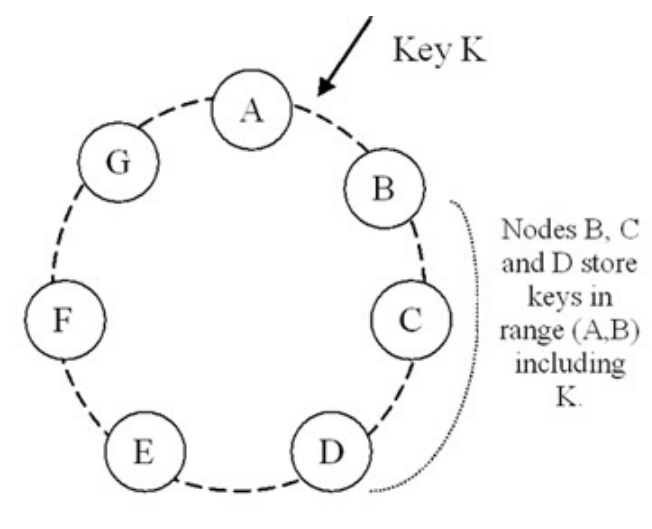
\includegraphics[width=\linewidth]{imgs/dynamo.png} 
\caption{Dynamo Architecture \& Key Lookup}\label{fig:1}
\end{wrapfigure} 

\textbf{Architecture:} All nodes communicate with each other through a Gossip protocol similar to Dynamo and Riak, exchanging information about themselves and other nodes they have gossiped with. It is a peer-to-peer system where all nodes are identical. This allows for many interesting features such as no single point of failure, ability to read/write to any node, and lineally scalable. O(1) looks-ups are provided by hashing the key to find out which servers have the needed information (Figure \ref{fig:1}).

\begin{wrapfigure}{l}{6.5cm}
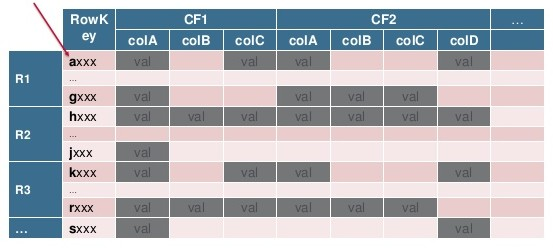
\includegraphics[width=\linewidth]{imgs/data_model.jpg} 
\caption{Cassandra Data Model}\label{fig:2}
\end{wrapfigure} 

\textbf{Data Model:} Cassandra’s data model, derived from Google’s BigTable, is a partitioned row datastore organized into tables, where the rows are key-value pairs. Each table contains a set of primary keys which uniquely identify each row of data. Columns in Cassandra are grouped into column family. It is considered schema-free because although the column families are defined, the columns are not. You can freely add any column to any column family at any time, depending on your needs. Another major difference between Cassandra and a relational database is that Cassandra's only datatype is byte array, similar to Apache HBase and Google BigTable. 

\textbf{Consistency}: An additional feature of Cassandra is its tunable data consistency. User can, per query, choose between strong consistency and eventual consistency to best fit their application design. This is done by choosing how many nodes to talk to for each read and write operation. For this example, say there are N replicas for data item x. Clients talk to R nodes for read operations and W nodes for write operations. Cassandra can provide strong consistency if R + W > N, but if the user is fine with occasionally receiving stale data, they can lower that requirement. This allows users to trade consistency for performance gains. \\
This also allows users to tune your queries depending on the type of work load they have. If most of the operations being performed are read operations, you can decrease R and increase W to decrease read latency, and vice versa for write operations.

\end{minipage} % End the main body - first page mini page

\end{document} 
